%%%%%%%%%%%%%%%%%%%%%%%%%%%%%%%%%%%%%%%%%%%%%%%%%%%%%%%
% Math 3250 Combinatorics, University of Connecticut
%%%%%%%%%%%%%%%%%%%%%%%%%%%%%%%%%%%%%%%%%%%%%%%%%%%%%%%

% Anything after a percent sign is a comment.

% Necessary first line. \documentclass defines the type of document and some options (for example, try changing the font size (10pt or 11pt or 12pt).
\documentclass[10pt]{amsart}
\usepackage{enumerate} % to be able to enumerate a list using non-numbers
\usepackage{tikz}
%for hypertext references
\usepackage[colorlinks = true,
            linkcolor = blue,
            urlcolor  = blue,
            citecolor = red,
            anchorcolor = green]{hyperref}


\usepackage[letterpaper]{geometry} % from 2016
\geometry{tmargin=0.93in,bmargin=-0.0in,lmargin=1.50in,rmargin=1.50in}
\voffset -0.5in

% The part of the tex file between the \documentclass and \begin{document} line is called the preamble.  Things having to do with setting up the document are done in the preamble.  You will not need to mess with it for now, except to change your name and the title of your document. 
% After adding your name next to author, head down to where it says "Start here"

\title{Math3250 Presentation Problems Week 2}
%\author{your preferred first and last name:}
%\date{due at the end of class on d2, Week 1}
\begin{document}

\maketitle

% --------------------------------------------------------
%                         Start here
% --------------------------------------------------------

%\noindent Credit: 
%Write down everyone who helped you, including classmates who contributed to your thought process. Write down Bona's textbook and other written sources you used as well.

\subsection*{Presentation Instruction}
The following problems may be chosen for presentation problems during class. 
If you have attempted the problem before class (even if you don't have complete solution), you can volunteer to present the problems in a group of size 1 or 2. 
You can also volunteer to earn audience participation that day instead. 


Reference the  \href{https://www.worldscientific.com/doi/pdf/10.1142/9789813148857_0001}{first chapter} and second chapter of  B\'ona's ``A Walk Through Combinatorics" textbook (4th, 3rd, or 2nd Ed.) for Pigeon-Hole Principle (the first \ref{sec:fridays} problems)  and induction methods (the rest of the problems).

\subsection*{Future homework and exam}
A subset of these presentation problems will be chosen for future homework and exam problems.

\bigskip



\section{Soccer Team} 
A soccer team scored a total of 40 goals this season. Nine players scored at least one of those goals. Prove that there are two players among those nine who scored the same number of goals.
\begin{proof}
\end{proof}



\section{Faculty members}
A college has $39$ departments, and a total of $262$ faculty members in those departments. Prove that there are three departments in this college that have a total of at least $21$ faculty members.
\begin{proof}
\end{proof}

\section{Five real numbers whose sum is $100$} 
Let's say I give you a mystery set of five positive real numbers whose sum is $100$. Prove that there are two numbers among them whose difference is at most $10$.

\begin{proof}
\end{proof}

\section{Fridays}\label{sec:fridays} 
The month of January 2020 has five Fridays. (Optional: How many months in 2020 contain five Fridays?) For any given year, use the Pigeon-hole Principle to determine the possible number of months that contain five Fridays.
See the source code for hints: 
%For any given year, there are either four or five months that contain five Fridays.\\ To answer this, consider: \\(i) How many Fridays are there in one year? \\(ii) Each month has at least 28 days, so each month has at least four Fridays.
\begin{proof}
Insert proof
\end{proof}




\section{polygon}
Prove (using induction) that the sum of the angles of a convex $n$-gon is $(n-2)180$ degrees.

Note: You may use the fact that the sum of angles of a convex triangle is $180^o$ without proof.
\begin{proof}
	Insert proof
\end{proof}


\section{Squares}
We start with one square piece of paper 
\begin{tikzpicture}[scale=1.2]
\draw(0,0) grid (1,1);
\end{tikzpicture}.

We then cut this square paper into four smaller squares
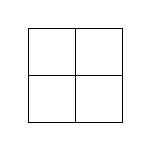
\begin{tikzpicture}[scale=0.6]
\draw(0,0) grid (2,2);
\end{tikzpicture}.

Then cut one of the obtained small squares into four smaller squares, so that we get $7$ squares 
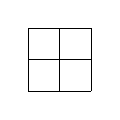
\begin{tikzpicture}[scale=0.4]
\draw(0,0) grid (2,2);
\end{tikzpicture} \hspace {-1cm}
\begin{tikzpicture}[scale=0.8]
\draw(1,1) grid (0,0);
\draw(1,1) grid (2,0);
\draw(1,0) grid (2,-1);
\end{tikzpicture}, 
and so on.

Let $a_n$ be the number of squares we have after the $n$-th time that we perform this cutting operation. 
Compute the first few values of $a_n$ (beyond $n=1$ and $n=2$ given above), then conjecture an explicit formula for $a_n$, and then prove the formula using induction.
\begin{proof}
	Insert proof
\end{proof}


\section{Recurrence Relation}

\subsection{Sample Solution}
Let the sequence $\{ a_n\}$ be defined by the relations $a_0=1$, and let
\[
a_{n+1} = 2(a_0 + a_1 + \dots + a_n) 
\]
for $n \geq 0$. 
Compute the first few values of $a_n$, then conjecture an explicit formula for $a_n$, and then prove the formula using induction.
\begin{proof}[Solution and proof]
	We claim that $a_n = 2 \cdot 3^{n-1}$ for $n \geq 1$. We prove this by strong induction on $n$.
	Since $2(a_0)=2(1)=2\cdot 3^{1-1}$, the initial case (for $n=1$) is verified.  
	Now let us assume that the statement is true for all positive integers that are less than or equal to $n$. Then, we have
	\begin{align*}
		a_{n+1} &= 2(a_0 + a_1 + a_2 + \dots + a_n) ~ \text{ by the recurrence relation}\\
		&= 2 a_0 + 2 (a_1 + a_2 + \dots +  a_n)\\
		&= 2 + 2(2 \cdot 1 + 2 \cdot 3 + \dots + 2 \cdot 3^{n-1}) ~ \text{ by the induction hypothesis}\\
		&= 2 + 4 ( 1 +  3 + \dots +  3^{n-1})\\
		&= 2 + 4 \left( \frac{3^n - 1}{2}  \right) ~ \text{ since the series is a geometric series} \\
		&= 2 + 2 (3^n - 1) \\
		&= 2 \cdot 3^n.
	\end{align*}
	This proves that our explicit formula is correct for $n+1$, and the proof is complete.
\end{proof}


\subsection{A recurrence relation problem}
Let the sequence $\{ a_n\}$ be defined by the relations $a_0=1$, and 
\[
a_n = 3(a_0 + a_1 + \dots + a_{n-1}) + 1
\]
for $n>0$. 
Compute the first few values of $a_n$, then conjecture an explicit formula for $a_n$, and then prove the formula using induction.

See hint in source code.
%hint: Use Sec 2.2 Strong Induction. Copy and paste the sample solution typed above.  Follow Example 2.5 and Example 2.6 in the book and also the sample solution typed above.

\begin{proof}
	Insert proof
\end{proof}


\section{Divisible by three}
\emph{Use strong induction} to prove that a positive integer is divisible by $3$ if and only if the sum of its digits is divisible by $3$.

\begin{proof}
	Insert proof
\end{proof}

\end{document}
